\chapter{Oscillations and Waves}

\section{Simple Harmonic Motion (S.H.M.)}

\subsection{Equation of Motion}

Consider the following systems.

\begin{center}
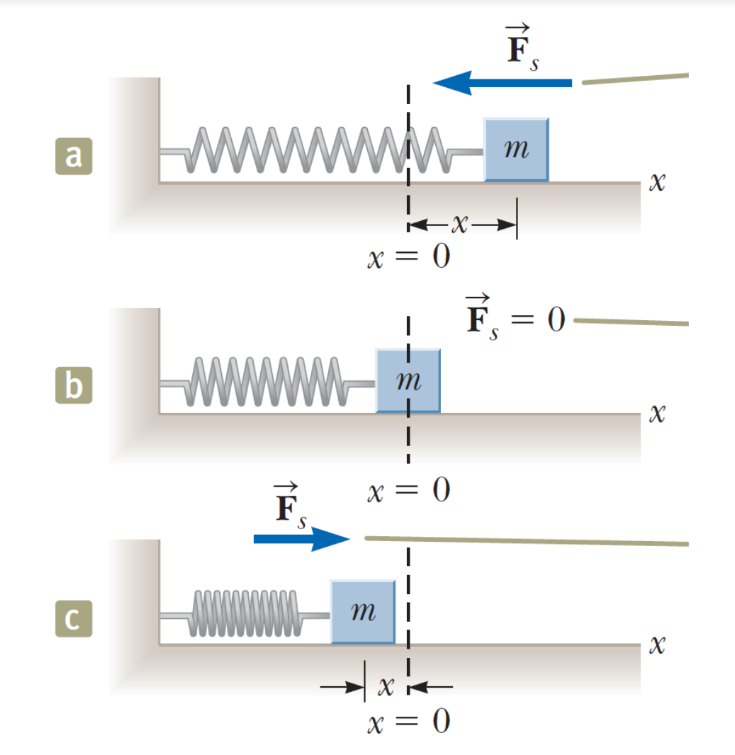
\includegraphics[scale=0.5]{oaw/spring01.png}
\end{center}

From Physics I, we know that we can use Hooke's Law to calculate the spring force. \[ \vec{F_s} = -kx \]

When the spring is stretched, $\vec{F_s}$ is negative. When the spring is at equilibrium,
$\vec{F_s} = 0$. If the spring is compressed, $\vec{F_s}$ is positive. There is only one force,
everything is in 1D, and everything is equal to $ma$ from Newton's $F = ma$. Thus, we can
derive the \textbf{Equation of Motion}. \[ \sum F_x = -kx = ma_x \]

In our equation, we can turn $a$ into $d^2x / dt^2$ since accerelation is just the second
derivative of displacement. Then, through some manipulation, we can derive
\[ -kx = ma_x = m\frac{d^2x}{dt^2} \implies \frac{d^2x}{dt^2} = -\frac{k}{m}x \]
which is a differential equation we need to solve. Now, what sort of function $x(t)$ do we 
use such that its second derivative would still contain an $x$ term and is negative?

We have a few choices: polynomic with negative power, exponential, logarithmic, and trigonometric
functions. Our choice? \textit{Trigonometric functions}, specifically $\sin$ and $\cos$. Finally,
we have found a suitable function $x$.

\[ x(t) = A\sin(\omega t + \phi) \]

We can also choose to use the $\cos$ function as well as they give the same result. Essentially,
we can convert between $\sin$ and $\cos$ since we have the $\phi$ term.

\subsection{Interpretation}

We can interpret $\omega$ as the angular frequency which is $2\pi f = 2\pi / T$.
Knowing that $\omega = \sqrt{k/m}$, this means that for a given spring with a certain $k$ and mass $m$,
we cannot change the way that it oscillates. No matter how much we stretch, it's going to bounce with
that frequency. This is called the \textbf{Natural Frequency}. The only way to change is to change 
the value of $k$ and $m$.

Simple Harmonic Motion refers to a motion with a single frequency $-$ $\omega$.
Obviously, there exists Harmonic Motion that are not simple. However, it is out of the scope of this course.

\subsection{Equation of Motion on a Pendulum}

\begin{center}
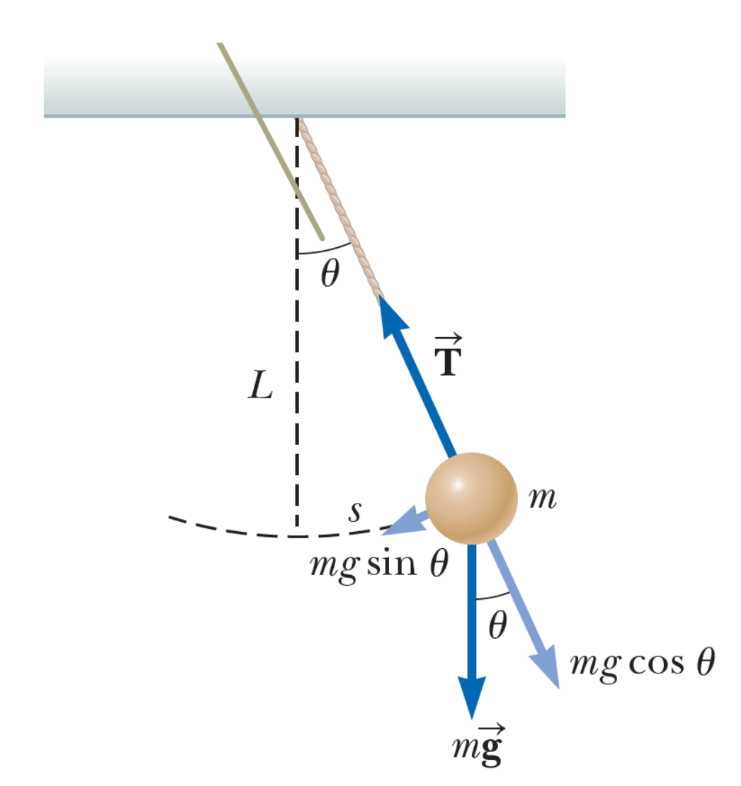
\includegraphics[scale=0.3]{images/oaw/pendulum01.png}
\end{center}

In order to analyze the motion of the pendulum, we can break down said motion into the vertical and
horizontal components. We can say that the tension $T = mg\cos\theta$ then completely ignore the motion's
vertical component as they cancel out. Therefore, the only remaining forces will be
\[\sum F_t = ma_t \implies -mg\sin\theta = m\frac{d^2s}{dt^2}\]
where $s$ is the tangential distance (displacement in circular motion). Once we cancel everything
and rearrange it such that it looks like our previous differential equation, we will get
\[ \frac{d^2s}{dt^2} = -g\sin\theta \]

This is where we need to face the harshness of reality. We cannot solve this equation, not without
a computer. However, we can use some approximation tricks to help us.

If the angle $\theta$ of swing is small, $\sin\theta \approx \theta$. We can also change $s$ into 
something easier to deal with. Since we know that $\theta = s/L$ where $L$ is the radius, we can
express $s$ as $\theta L$. With some manipulation, our equation then becomes
\[ \frac{d^2(\theta)}{dt^2} \approx -\frac{g}{L}\theta \]

Therefore, the (approximate) solution to this equation of motion is
\[ \theta(t) = A\sin(\omega t + \delta), \omega = \sqrt{\frac{g}{L}} \]

In this case, mass does not even matter to the oscillation. The only things that matter are the 
gravitational accerelation ($g$) and the length of the string attached to your pendulum ($L$).
Interestingly, this was how people made clocks back in the day.

\subsection{Equation of Motion on Rotation}

\begin{center}
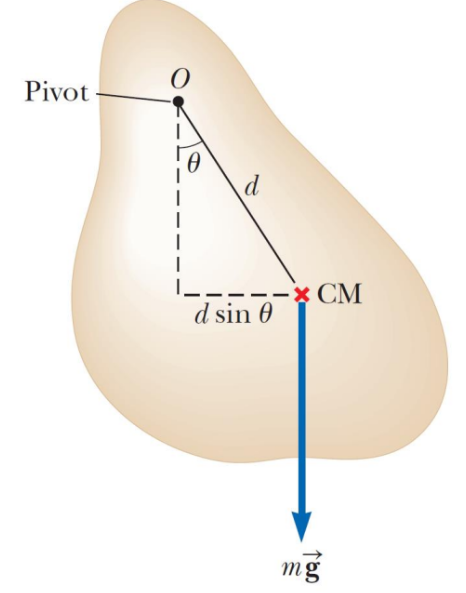
\includegraphics[scale=0.5]{images/oaw/rotation01.png}
\end{center}

Instead of Newton's equation, we now use $\vec{\tau} = I\vec{\alpha} = \vec{r}\times\vec{F}$.
From the diagram, we can see that the only thing generating torque is $m\vec{g}$. Let $r$ be the
distance from the pivot to the force (note that this distance is measured from $O$ to the point
perpendicular to the force), $r = d\sin\theta$. Now, torque will become $dmg\sin\theta$. Since
the torque is going clock-wise, the sign is negative. With some manipulation, our final 
approximate solution becomes
\[ \frac{d^2\theta}{dt^2} \approx -\frac{mgd}{I}\theta \]

Again, we can see that this is another simple harmonic motion where $\omega = \sqrt{(mgd)/I}$.

\subsection{Energy of Simple Harmonic Oscillator}

We can first find the kinetic and potential energy by
\begin{align*}
    K &= \frac{1}{2}mv^2 = \frac{1}{2}m\omega^2A^2\sin^2(\omega t + \phi)\\
    U &= \frac{1}{2}kx^2 = \frac{1}{2}A^2\cos^2(\omega t + \phi)
\end{align*}

Then, we can derive the total energy by
\begin{align*}
    E &= K + U\\
    &= \frac{1}{2}m\omega^2A^2\sin^2(\omega t + \phi) + \frac{1}{2}A^2\cos^2(\omega t + \phi)\\
    &= \frac{1}{2}kA^2 ( \sin^2(\omega t + phi) + \cos^2(\omega t + phi))\\
    &= \frac{1}{2}kA^2
\end{align*}
Note that since $\omega^2 \ k / m$, $(1/2)m(k/m) = (1/2)k$.

What does this mean? At any moment in time, the sum of the energy of the system must remain the same.
This aligns with the conservation of energy.